% Created 2022-02-12 Sat 17:47
% Intended LaTeX compiler: pdflatex
\documentclass[presentation,aspectratio=169]{beamer}
\usepackage[utf8]{inputenc}
\usepackage[T1]{fontenc}
\usepackage{graphicx}
\usepackage{grffile}
\usepackage{longtable}
\usepackage{wrapfig}
\usepackage{rotating}
\usepackage[normalem]{ulem}
\usepackage{amsmath}
\usepackage{textcomp}
\usepackage{amssymb}
\usepackage{capt-of}
\usepackage{hyperref}
\usepackage{khpreamble, euscript}
\DeclareMathOperator{\atantwo}{atan2}
\newcommand*{\ctrb}{\EuScript{C}}
\newcommand*{\obsv}{\EuScript{O}}
\usetheme{default}
\author{Kjartan Halvorsen}
\date{\today}
\title{The unicycle model}
\hypersetup{
 pdfauthor={Kjartan Halvorsen},
 pdftitle={The unicycle model},
 pdfkeywords={},
 pdfsubject={},
 pdfcreator={Emacs 26.3 (Org mode 9.4.6)}, 
 pdflang={English}}
\begin{document}

\maketitle

\section{Mobile robot unicycle model}
\label{sec:org9072577}

\begin{frame}[label={sec:org381172e}]{The unicycle model}
\begin{columns}
\begin{column}{0.4\columnwidth}
\begin{center}
 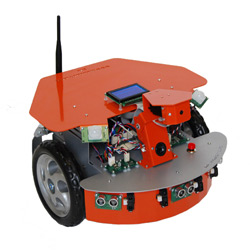
\includegraphics[width=.3\linewidth]{../figures/X80Pro.jpg}
\end{center}
\begin{center}
 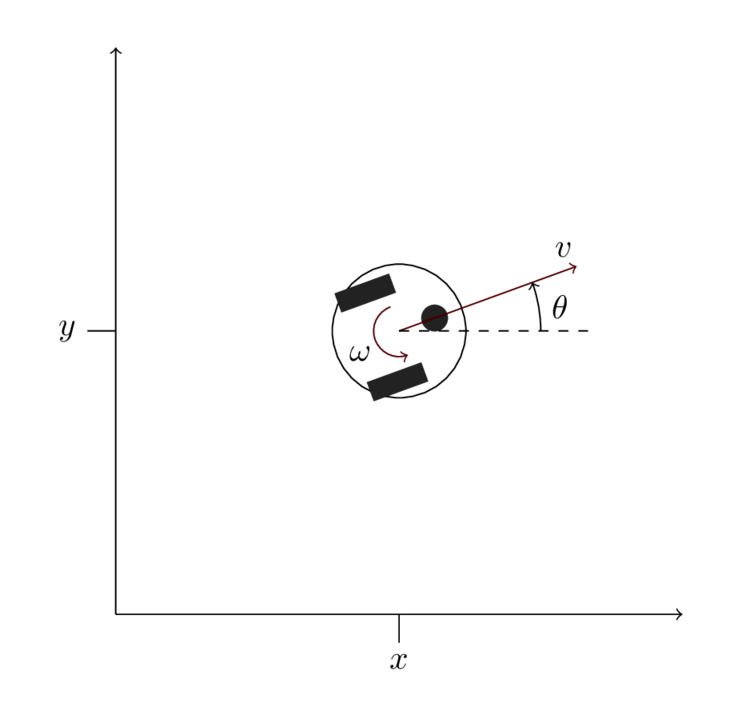
\includegraphics[width=1.0\linewidth]{../figures/unicycle-model}
\end{center}
\end{column}

\begin{column}{0.6\columnwidth}
\pause

\[ \xi = \begin{bmatrix} \theta\\x\\y \end{bmatrix},   \quad u = \begin{bmatrix} \omega\\v \end{bmatrix}\]



\[\frac{d}{dt} \xi = \begin{bmatrix} \dot{\theta}\\\dot{x}\\\dot{y} \end{bmatrix} = \begin{bmatrix} \omega\\ v\cos\theta\\v\sin\theta\end{bmatrix} \]

Called unicycle model.
\pause

\alert{Activity} Can we reach any point in state space \(\begin{bmatrix} x &  y & \theta \end{bmatrix}^T\) by a suitably designed input signal sequence \(u(t)\)?
\end{column}
\end{columns}
\end{frame}

\begin{frame}[label={sec:orgc902816}]{The unicycle model}
\small 
\begin{columns}
\begin{column}{0.4\columnwidth}
\begin{center}
 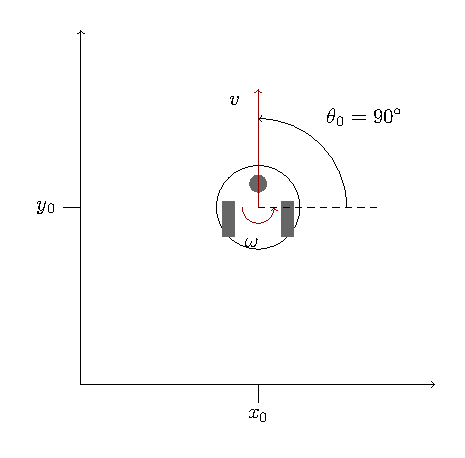
\includegraphics[width=1.0\linewidth]{../figures/unicycle-model-op}
\end{center}

\[\frac{d}{dt} \xi = \begin{bmatrix} \dot{\theta}\\\dot{x}\\\dot{y} \end{bmatrix} = \begin{bmatrix} \omega\\ v\cos\theta\\v\sin\theta\end{bmatrix} \]
\end{column}
\begin{column}{0.6\columnwidth}
Linearized model using deviation variables
\[ \xi(t) = \xi_0 + z(t), \quad \frac{d}{dt} \xi = \frac{d}{dt} z\]
\[ \frac{d}{dt} z = \begin{bmatrix} \omega\\ v\cos\theta_0 \\ v\sin\theta_0 \end{bmatrix}
= \underbrace{0}_{A} z + \underbrace{\begin{bmatrix} 1 & 0 \\ 0 & 0\\ 0 & 1\end{bmatrix}}_{B} \begin{bmatrix}\omega\\v\end{bmatrix} \]

\pause

\begin{align*} \mathcal{C} &= \begin{bmatrix} B & AB & A^2B \end{bmatrix}\\
&= \begin{bmatrix} 1 & 0 & 0 & 0 & 0 & 0 \\ 0 & 0 & 0 & 0 & 0 & 0\\ 0 & 1 & 0 & 0 & 0 & 0\end{bmatrix}
\end{align*}

\pause

\alert{Activity} Is the linearized model controllable? (Hint: What is \(\text{rank}\, \mathcal{C}\)?)
\end{column}
\end{columns}
\end{frame}
\end{document}